%!TEX program = xelatex
\documentclass[a4paper,UTF8]{ctexart}

\usepackage{fontspec}
\usepackage{amsmath}
\usepackage{float}
\usepackage{graphicx}
\usepackage{amssymb}
\usepackage{epstopdf}
\usepackage{mathrsfs}
%\usepackage{stmaryrd}
\usepackage{color}
\usepackage{listings}
\usepackage{ulem}
\usepackage{lmodern}
\usepackage{fontenc}
\usepackage[margin=2cm]{geometry}
\usepackage{titlesec}
%\usepackage{svg}
\usepackage{tikz}
\usepackage{hyperref}
\usepackage[noblocks]{authblk}

\setlength{\parskip}{5pt}

\usepackage{MyTitle}
\titleformat{\section}[hang]{\bfseries\fontsize{16pt}{0pt}\selectfont}{\thesection}{.5em}{}{}


% 对于使用 Tex Pad 打开本 TeX 文档的用户,请使用这行代码
\usepackage[cache=false,outputdir=.texpadtmp]{minted}
% 其它用户使用这行
%\usepackage{minted}
%

%To do: 修改标题和作者及联系方式
\title{HITCON2015 Quals, Reverse300, risky}

\author{黄清水(Skyner)}
\affil{哈尔滨工业大学,软件学院,skyner@foxmail.com}

\date{}

\begin{document}
\maketitle

\begin{center}
\parbox{0.9\textwidth}{
\textbf{摘~~~要}\quad 本文是 HITCON2015 Quals 比赛,risky一题的题解,主要介绍了本题的解题思路和解题方法,本题解参考并引用了匈牙利!SpamAndHex战队关于此题的题解\cite{writeup}。同时本题解探讨了面对非常见指令集程序的应对方法。\\
\textbf{关键词}\quad HITCON, CTF, Reverse, Social Engineering, RISC-V\\}
\end{center}


%------------------------------------------------------------------------------------------------------------------------------
%------------------------------------------------------------------------------------------------------------------------------
%To do: 正文开始
%------------------------------------------------------------------------------------------------------------------------------
%------------------------------------------------------------------------------------------------------------------------------

\section{题目描述}

本题是逆向工程学范畴一道分值为 100 的题目,其描述如下:\\

\begin{quizdesc}[label=Reverse300 risky]
RISKY machine

risky-13de1366628df39000749a782f69d894
\end{quizdesc}

本题题干除了RISKY machine这个不能更简短的描述以外,就是一个elf格式文件。

\section{解题思路}

\subsection{尝试常规手段用IDA分析}
将此文件下载后拖入IDA分析,得到结果如下:

\begin{figure}[hbt!]
  \centering
  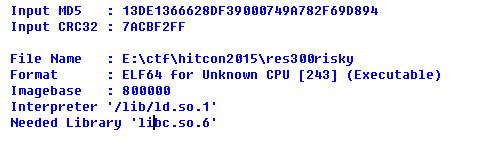
\includegraphics[width=0.80\textwidth]{idaview1.png}
  \caption{IDA分析结果1}\label{idaview1}
\end{figure}

\begin{figure}[hbt!]
  \centering
  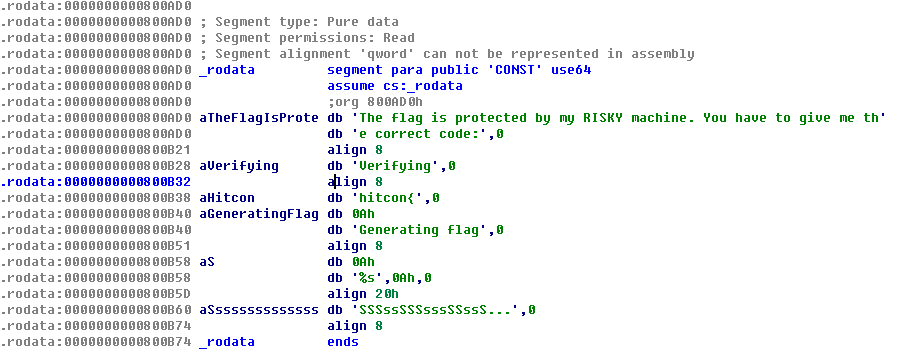
\includegraphics[width=0.80\textwidth]{idaview2.png}
  \caption{IDA分析结果2}\label{idaview2}
\end{figure}

通过IDA分析,得到的有效信息仅限于如上两图,从图 \ref{idaview1} 中仅能得知这是个64位的linux程序,而这个程序所用到的machine居然是unknown…… 在图 \ref{idaview2} 中可以看到一些程序数据段中储存的预设字符串信息,作者告诉我们flag被保护在了risky machine,这是第二次出现这个词了,那么这个risky machine到底是什么东西呢。结合代码段分析结果是一堆乱码,IDA无法识别该程序的指令集,可以初步得出结论,这个程序用了某种未知的指令集,这个指令集还会和risky这个词有关。

试着在linux中运行这个程序,果然,这个程序在linux 系统下无法运行。在终端中试图运行的结果是提示:无法执行二进制文件。然后我在linux kali 1.1 中使用 readelf -a 命令查看了文件的格式信息,仅仅得到两条有效信息:

\begin{quizdesc}
  OS/ABI:                            UNIX - System V

  Machine:                           <unknown>: 0xf3
\end{quizdesc}

\subsection{找办法确定程序所用指令集}

machine信息是在IDA中就已经知道了,还可以看到程序编译的操作系统环境为UNIX - System V。我在解题的时候谷歌搜索了一下risky 这个词,并没有在搜索结果中发现什么有意义的信息出现。然后又试图从文件本身出发,首先搜索了UNIX系统下Machine特征值的含义,结果发现这个编号是保留字……,最后又试图从操作系统层面解决这个问题,查找UNIX - System V所支持的指令集系统,结果根本没找到相关的列表。到这里,我就无解了……后来比赛结束后学习了!SpamAndHex关于此题的题解,发现这是个risc-v程序!这里应该是因为英文素养的不足导致对risky一词的不敏感。
在英语中k与c的发音常常相同,y可视为v的变形,这词其实就是risc-v的变形,其实只要搜索risc就可以在谷歌搜索中得到risc-v官网的搜索结果(\url{http://riscv.org/}),所以在遇到未知指令格式文件的时候要善于利用社工手段分析题目中给予的信息,一般题目中总会通过某种方式给予提示。

在官网中我们终于找到了这个程序的运行方法,在官网中可以找到相关的运行支持工具\cite{risc_tools},包括了Linux下的反汇编工具以及动态运行环境。但是因为没有办法通过官网提供的工具进行内存和CPU寄存器层面的动态跟踪调试,所以只能对程序进行静态分析。risc-v官网同样提供了相关的支持文档\cite{risc_doc}。

\section{解题过程}

\subsection{第一步:粗略浏览整个程序}

粗略浏览整个程序后可以发现这个程序的机制是程序会从输入中读取一段连续的字符串然后检查该字符串是否正确,若正确则将该字符串打印为flag。

\subsection{第二步:分析字符串校验方式}

通过分析可以确定该程序提示程序首先提示用户输入,并且确保输入格式是\code{XXXX-XXXX-XXXX-XXXX-XXXX}。相关汇编码如下:

\begin{minted}{text}
8005cc:       02d00693                li      a3,45
800610:       0097c683                lbu     a3,9(a5)
800614:       fce692e3                bne     a3,a4,8005d8 <.exit>
800618:       00e7c703                lbu     a4,14(a5)
80061c:       fad71ee3                bne     a4,a3,8005d8 <.exit>
800620:       0137c603                lbu     a2,19(a5)
800624:       fae61ae3                bne     a2,a4,8005d8 <.exit>
800628:       0187c683                lbu     a3,24(a5)
80062c:       00a00713                li      a4,10
800630:       fae694e3                bne     a3,a4,8005d8 <.exit>
\end{minted}

然后检查字符串是否仅仅只包含\code{'-'}字符、大小写字母和数字。

\begin{minted}{text}
800648:       0006c703                lbu     a4,0(a3)
80064c:       00168693                addi    a3,a3,1
800650:       fd37071b                addiw   a4,a4,-45
800654:       0ff77713                andi    a4,a4,255
800658:       00e855b3                srl     a1,a6,a4
80065c:       0015f593                andi    a1,a1,1
800660:       f6e66ce3                bltu    a2,a4,8005d8 <.exit>
800664:       fc059ee3                bnez    a1,800640 <.next_check>
800668:       f71ff06f                j       8005d8 <.exit>
\end{minted}

这些都完成以后,将这五段字符中的每一段分别载入寄存器,并视作一个32位整数,并检查他们是否符合一系列等式。

\begin{minted}{text}
800694:       03548b3b                mulw    s6,s1,s5
800698:       181aa737                lui     a4,0x181aa
80069c:       c5f7071b                addiw   a4,a4,-929
8006a0:       032987bb                mulw    a5,s3,s2
8006a4:       016787bb                addw    a5,a5,s6
8006a8:       008787bb                addw    a5,a5,s0
8006ac:       f2e796e3                bne     a5,a4,8005d8 <.exit>
\end{minted}

可以将这段汇编代码翻译成如下形式:

\begin{minted}{c}
w0 * w1 + w2 * w3 + w4 == (0x181aa << 12) - 929
w0 * w2 + w1 + w4 == (0x2dead << 12) - 821
w0 + w1 + w2 + w3 + w4 == (0x8e2f6 << 12) + 1920
(w1 + w2 + w4) * (w0 + w3) == (0xb3da8 << 12) - 1185
w1 + w2 + w4 == (0xe3b0d << 12) - 529
w0 * w4 == (0x4978e << 12) - 1980
w1 * w2 == (0x9bcd3 << 12) + 222
w1 * w2 * w2 * w3 * w4 == (0x41c7a << 12) + 928
w2 * w3 == (0x313ac << 12) + 1924
\end{minted}

如果所有约束条件被满足,那么五段字符串将会异或一些预设的常数,然后拼接成一段字符串,并将得到的结果作为flag输出。

用Python \code{z3}跑出符合约束条件的字符串为:\code{KTIY-ML5M-VK7R-FE5Q-L6DD}。

异或操作的汇编码如下:

\begin{minted}{text}
80080c:       2c2817b7                lui     a5,0x2c281
800810:       d2f7879b                addiw   a5,a5,-721
800814:       02f12023                sw      a5,32(sp)
800818:       380537b7                lui     a5,0x38053
80081c:       5257879b                addiw   a5,a5,1317
800820:       02f12223                sw      a5,36(sp)
800824:       6b5c37b7                lui     a5,0x6b5c3
800828:       a247879b                addiw   a5,a5,-1500
80082c:       02f12423                sw      a5,40(sp)
800830:       275427b7                lui     a5,0x27542
800834:       7287879b                addiw   a5,a5,1832
800838:       02f12623                sw      a5,44(sp)
80083c:       297557b7                lui     a5,0x29755
800840:       72f7879b                addiw   a5,a5,1839
800844:       02f12823                sw      a5,48(sp)
\end{minted}

最后得到flag:\code{hitcon\{dYauhy0urak9nbavca1m\}}

\subsection{使用到的脚本}

下面这段 python 脚本可以求出flag。

\begin{minted}{python}
from z3 import *

s = Solver()

serial = []
serial.append(BitVec('serial_0', 32))  # X
serial.append(BitVec('serial_1', 32))  # X
serial.append(BitVec('serial_2', 32))  # X
serial.append(BitVec('serial_3', 32))  # X
serial.append(BitVec('serial_4', 32))  # -
serial.append(BitVec('serial_5', 32))  # X
serial.append(BitVec('serial_6', 32))  # X
serial.append(BitVec('serial_7', 32))  # X
serial.append(BitVec('serial_8', 32))  # X
serial.append(BitVec('serial_9', 32))  # -
serial.append(BitVec('serial_10', 32)) # X
serial.append(BitVec('serial_11', 32)) # X
serial.append(BitVec('serial_12', 32)) # X
serial.append(BitVec('serial_13', 32)) # X
serial.append(BitVec('serial_14', 32)) # -
serial.append(BitVec('serial_15', 32)) # X
serial.append(BitVec('serial_16', 32)) # X
serial.append(BitVec('serial_17', 32)) # X
serial.append(BitVec('serial_18', 32)) # X
serial.append(BitVec('serial_19', 32)) # -
serial.append(BitVec('serial_20', 32)) # X
serial.append(BitVec('serial_21', 32)) # X
serial.append(BitVec('serial_22', 32)) # X
serial.append(BitVec('serial_23', 32)) # X
serial.append(BitVec('serial_24', 32)) # \n

# a6 = BitVec('a6', 64)
# s.add(a6 == 0x0000ff3ff0fff91f)

# Check serial format
# Check for colons
s.add(serial[4] == 0x2d)
s.add(serial[9] == 0x2d)
s.add(serial[14] == 0x2d)
s.add(serial[19] == 0x2d)
s.add(serial[24] == 0x10)

# Check for charset
for i in range(24):
    s.add(serial[i] >= 0x2d)
    s.add(serial[i] <= 0x5a)

    charset = [45, 48, 49, 50, 51, 52, 53, 54, 55, 56, 57, 65, 66, 67, 68, 69, 70, 71, 72, 73, 74, 75, 76, 77, 78, 79, 80, 81, 82, 83, 84, 85, 86, 87, 88, 89, 90]
    expr = (serial[i] == charset[0])
    for char in charset[1:]:
        expr = Or(expr, serial[i] == char)

    s.add(expr == True)

words = []
w0 = (serial[0] +
    serial[1] * 0x100 +
    serial[2] * 0x10000 +
    serial[3] * 0x1000000)
w1 = (serial[5] +
    serial[6] * 0x100 +
    serial[7] * 0x10000 +
    serial[8] * 0x1000000)
w2 = (serial[10] +
    serial[11] * 0x100 +
    serial[12] * 0x10000 +
    serial[13] * 0x1000000)
w3 = (serial[15] +
    serial[16] * 0x100 +
    serial[17] * 0x10000 +
    serial[18] * 0x1000000)
w4 = (serial[20] +
    serial[21] * 0x100 +
    serial[22] * 0x10000 +
    serial[23] * 0x1000000)

# Check products
s.add(w0 * w1 + w2 * w3 + w4 == (0x181aa << 12) - 929)
s.add(w0 * w2 + w1 + w4 == (0x2dead << 12) - 821)
s.add(w0 + w1 + w2 + w3 + w4 == (0x8e2f6 << 12) + 1920)
s.add((w1 + w2 + w4) * (w0 + w3) == (0xb3da8 << 12) - 1185)
s.add(w1 + w2 + w4 == (0xe3b0d << 12) - 529)
s.add(w0 * w4 == (0x4978e << 12) - 1980)
s.add(w1 * w2 == (0x9bcd3 << 12) + 222)
s.add(w1 * w2 * w2 * w3 * w4 == (0x41c7a << 12) + 928)
s.add(w2 * w3 == (0x313ac << 12) + 1924)

if s.check() == sat:
    print "sat :)"
    m = s.model()

    res = ""
    serial_num = []

    for i in range(24):
        res += chr(int(str(m[serial[i]])))
        serial_num.append(int(str(m[serial[i]])))

    print res

    w0 = (serial_num[0] +
        serial_num[1] * 0x100 +
        serial_num[2] * 0x10000 +
        serial_num[3] * 0x1000000)
    w1 = (serial_num[5] +
        serial_num[6] * 0x100 +
        serial_num[7] * 0x10000 +
        serial_num[8] * 0x1000000)
    w2 = (serial_num[10] +
        serial_num[11] * 0x100 +
        serial_num[12] * 0x10000 +
        serial_num[13] * 0x1000000)
    w3 = (serial_num[15] +
        serial_num[16] * 0x100 +
        serial_num[17] * 0x10000 +
        serial_num[18] * 0x1000000)
    w4 = (serial_num[20] +
        serial_num[21] * 0x100 +
        serial_num[22] * 0x10000 +
        serial_num[23] * 0x1000000)

    x0 = (0x2c281 << 12) - 721
    x1 = (0x38053 << 12) + 1317
    x2 = (0x6b5c3 << 12) - 1500
    x3 = (0x27542 << 12) + 1832
    x4 = (0x29755 << 12) + 1839

    s0 = ("%08x" % (w0 ^ x0)).decode('hex')[::-1]
    s1 = ("%08x" % (w1 ^ x1)).decode('hex')[::-1]
    s2 = ("%08x" % (w2 ^ x2)).decode('hex')[::-1]
    s3 = ("%08x" % (w3 ^ x3)).decode('hex')[::-1]
    s4 = ("%08x" % (w4 ^ x4)).decode('hex')[::-1]

    print "hitcon{%s%s%s%s%s}" % (s0, s1, s2, s3, s4)

else:
    print "unsat :("

\end{minted}

\begin{thebibliography}{99}
\setlength{\parskip}{0pt}  %段落之间的竖直距离

\bibitem{writeup} !SpamAndHex write up, \url{https://kt.pe/blog/2015/10/hitcon-2015-quals-risky/}
\bibitem{riscv_tools} riscv-tools, \url{http://riscv.org/download.html#tab_tools}
\bibitem{riscv_doc} riscv User-Level ISA Specification v2.0, \url{http://riscv.org/spec/riscv-spec-v2.0.pdf}
\end{thebibliography}

%------------------------------------------------------------------------------------------------------------------------------
%OK: 正文结束
%------------------------------------------------------------------------------------------------------------------------------


\end{document}
